%\documentclass[11pt]{article}
\documentclass[print,phd]{nuthesis}
%\usepackage{times}

%\setlength{\textwidth}{6.5in}
%\setlength{\textheight}{9.0in}
%\setlength{\topmargin}{-.5in}
%\setlength{\oddsidemargin}{-.0600in}
%\setlength{\evensidemargin}{.0625in}

\newcommand{\secref}[1]{Section~\ref{#1}}
\usepackage{xcolor}
\usepackage{setspace}
%\usepackage{algorithmic}
\usepackage{amsmath}
\usepackage{amssymb}
\usepackage{cite}
\usepackage{textcomp}
\usepackage{float}
\usepackage{caption}
%\usepackage{algorithm}
\usepackage{url}
%SPAWC-2018
\usepackage{color}
\usepackage{enumitem}


\usepackage[pdftex]{graphicx}
\usepackage{graphicx}
\usepackage{calc}
\usepackage{url}
\usepackage{listings}
\usepackage{subfig}
\usepackage{multirow}
\usepackage{bbding}
\usepackage{rotating}
\usepackage{array}
\usepackage{float}

%SPAWC-2018
\usepackage{graphics}
\usepackage{mathtools}
\usepackage{bigints}
\usepackage{float}
\usepackage{caption}
%\usepackage{subcaption}
\usepackage[ruled, linesnumbered]{algorithm2e}
%\usepackage[linesnumbered,lined,boxed,commentsnumbered]{algorithm2e}
\usepackage{algpseudocode}
\usepackage[pdftex]{graphicx}
\usepackage{epstopdf}
\graphicspath{{./figures/}}
\usepackage[version=4]{mhchem}

\newlength{\imgwidth}

\newcommand\scalegraphics[1]{%   
    \settowidth{\imgwidth}{\includegraphics{#1}}%
    \setlength{\imgwidth}{\minof{\imgwidth}{\textwidth}}%
    \includegraphics[width=\imgwidth]{#1}%
}

% Haluk start
\usepackage[english]{babel}

\addto\captionsenglish{% Replace "english" with the language you use
  \renewcommand{\contentsname}%
    {\fontsize{14pt}{14}\bfseries Table of Contents}%
\renewcommand{\listfigurename}{\fontsize{14pt}{14}\bfseries List of Figures}
\renewcommand{\listtablename}{\fontsize{14pt}{14}\bfseries List of Tables}
}



\usepackage{anyfontsize}
\usepackage{titlesec}    

\titleformat{\chapter}[display]{\fontsize{14pt}{14}\bfseries}{Chapter \thechapter}{14pt}{\fontsize{14pt}{14}\bfseries}

\titleformat*{\section}{\fontseries{b}\fontsize{12pt}{12}\selectfont}
\titleformat*{\subsection}{\fontseries{b}\fontsize{11pt}{11}\selectfont}
\titleformat*{\subsubsection}{\fontseries{b}\fontsize{10pt}{10}\selectfont}


% Haluk end

%\doublespacing

%\author{Derek Weitzel\\
%Computer Science and Engineering\\
%University of Nebraska--Lincoln\\
%Lincoln, NE 66588-0115\\
%dweitzel@cse.unl.edu
%       }
\begin{document}
\frontmatter
\title{{\fontsize{12}{14}\selectfont Molecular Communication in Biological Cells: Foundational Study and Development of Computational Techniques}}
\author{Zahmeeth Sayed Sakkaff}
%\adviser{Dr. Massimiliano Pierobon, Chair \\ Dr. Myra B. Cohen \\ %Dr. Juan Cui \\ Dr. Tomas Helikar \\ Dr. Christopher S Henry}
\adviser{Under the Supervision of Professor Massimiliano Pierobon}

\adviserAbstract{Massimiliano Pierobon}
\major{Engineering}
\specialization{(Computer Engineering-Computer Science)}
\degreemonth{July}
\degreeyear{2019}
\maketitle

%%%ABSTRACT%%%
\begin{abstract}
\label{sec:summary}

\par Your abstract
\end{abstract}



%%%Acknowledgments%%%
\begin{acknowledgments}
\label{sec:ack}

\par Your ack
\end{acknowledgments}

%\newpage
\begin{KeepFromToc}
  \tableofcontents
\end{KeepFromToc}

\newpage
\listoffigures
\listoftables

% \doublespace
\mainmatter

%%% Chapter 01 - Introduction %%%
\chapter{Introduction}
\label{sec:Introduction}
\par Your intro

%Cite references
Reference ~\cite{Mahner08}. \\
Refere section or subsetion~\ref{lBackground}.\\
Equations ~\eqref{eqn:doane_formula}.

%%% Chapter 02 - Background %%%
\chapter{Background}
\label{sec:Background}

\section{Motivation}
\label{sec:motivation}
\par Your background

\section{Biological Pathways}
\label{sec:biologicalpathways}

%figures
\par 
\begin{figure} [h]
	\begin{center}
		\centering
		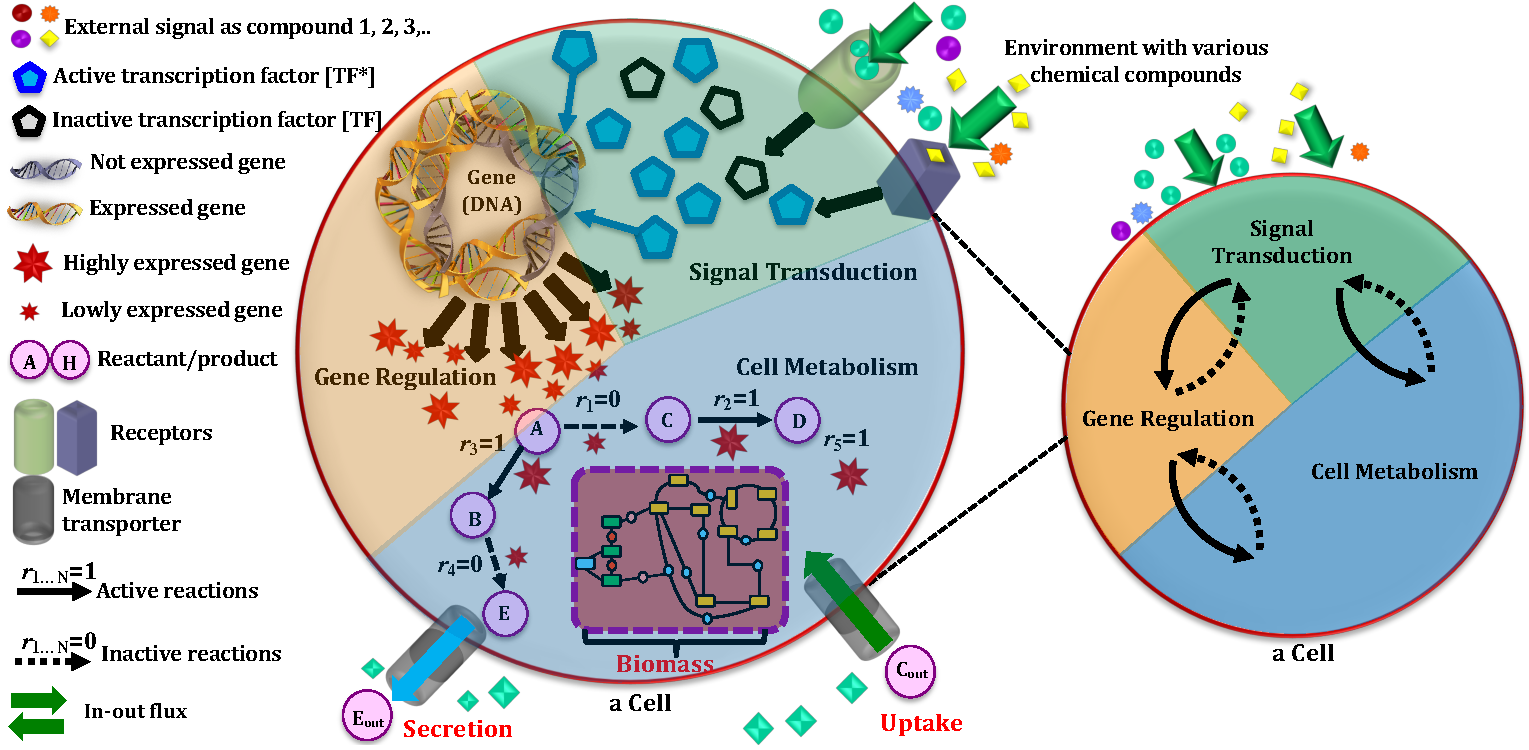
\includegraphics[width=\linewidth]{figures/E2E_model.pdf}
		\caption{Graphical representation of the interconnection of signal transduction, gene regulation and metabolic pathways.}
		\label{fig:biologicalpathways_1}
	\end{center}
\end{figure}

\subsection{Gene Regulation}
\label{subsec:generegulation}

%equations
\begin{equation} \label{eqn:doane_formula}
N_{j,t_n} = 1 + \log_2 (C) + \log_2 \left( 1+\frac{g_{Y_j(t_n)}}{\sigma_{g_{Y_j(t_n)}}} \right) \, .
\end{equation}

% algorithms
\begin{algorithm}[t!]
{\footnotesize
\KwData{$R$ simulation runs for each of $I$ input concentrations containing values for all $N$ simulation steps}
 \KwResult{For each protein $j$, $p_{Y_j}$ and $p_{X|\left\{ y_{j,t_n} \right\}_{n=0}^{N}}$}
\For{each simulation time step $t_n$}{
Create $\left\{Z_{i,r}\right\}_{t_n}$ by extracting protein $j$ concentration for each simulation run $r$ and input concentration $i$\\
Map each value of $\left\{Z_{i,r}\right\}_{t_n}$ in $N_{j,t_n}$ equally-spaced bins (with index $b_{t_n}$) between min and max values, expressed as $\left( \left\{Z_{i,r}\right\}_{t_n}, b_{t_n} \right) $ \\
}
Obtain matrix $M$ of size $C$ by $N$ by combining all the mapped bin indices $b_{t_n}$ for each simulation run $(i,r)$ and each time step $t_n$\\
Compute the multidimensional histogram considering each row of M as a datapoint: $p_{Y_j} \left( \left\{ y_{j,t_n} \right\}_{n=0}^{N} \right)$\\
\For{each bin in the multidimensional histogram}{
Take all the input values corresponding to the values $\left\{ y_{j,t_n} \right\}_{n=0}^{N}$ that define the current multidimensional bin\\
Compute the histogram $p_{X|\left\{ y_{j,t_n} \right\}_{n=0}^{N}}$ by mapping the input values found at Step 8 into $S_{\left\{ y_{j,t_n} \right\}_{n=0}^{N}}$ equally space bins between min and max values\\
If no input value from Step 8, set $p_{X|\left\{ y_{j,t_n} \right\}_{n=0}^{N}} = 0$ 
}
}
\caption{Probability Histograms for Equation~\eqref{eqn:est_conditional_entropy}}
\label{alg:MIAlg}
\end{algorithm}

%tables
\begin{table} [H]
\centering
\footnotesize{
	%\vspace{-0.2cm}
  \caption{Mutual information values for different sugars.}
  %	\vspace{-0.2cm}
    \centering
    
    \begin{tabular}{ |c|c|c|c| } 
\hline
Sugar Type & \footnotesize $\tilde{H}(X)$ & \footnotesize $\tilde{H}(X|bm(t_c))$ & \footnotesize $\tilde{H}(X)-\tilde{H}(X|bm(t_c))$ \\
\hline
  Glucose & 6.6295 & 5.2694 & 1.3601\\ 
 Lactose & 6.6295 &  5.2851 & 1.3444\\ 
 Glucose6P & 6.6295 &  5.8971 & 0.7324\\ 
\hline
\end{tabular}
    \label{tab:mi}
    	%\vspace{-0.6cm}%
    	}
\end{table}


\chapter{Conclusion and Future Directions}
\label{sec:Conclusion_FD}

\par Your conclusion
 
 \begin{itemize}
 \item AAA
    
 \item BBB
\end{itemize}
\backmatter

\bibliographystyle{plain}
\bibliography{ZSDissertation}

\end{document}

\endinput

